\section{Patterns: Design and Implementation}
\label{section:patterns}

In this section we will introduce the \emph{patterns} which form the expressions used for code generation.
As we saw in the previous section there exist two type of patterns: high-level algorithmic patterns and low-level \OpenCL patterns.
Some of the high-level algorithmic patterns directly correspond to algorithmic skeletons we have introduced in \autoref{chapter:skelcl}.
As we will also introduce patterns which we have not seen so far and which do not confirm to the common definition of algorithmic skeletons we will use the more generic term \emph{pattern} throughout this and the next chapter.

The key idea of our approach is to expose algorithmic choices and hardware-specific program optimizations as patterns that are systematically derived using a rule rewriting system (discussed later in \autoref{section:rules}).
The high-level algorithmic patterns represent structured parallelism.
They can either be used by the programmer directly as a stand-alone language (or embedded DSL) or used as an intermediate representation targeted by another language.
Once a program is represented with our high-level patterns, we automatically transform the program into low-level patterns.
The low-level hardware patterns represent hardware specific concepts expressed by a programming model such as \OpenCL, the target chosen for this thesis.
Following the same approach, a different set of low-level patterns could be designed to target other low-level programming models such as Pthreads or MPI.


\subsection{High-level Algorithmic Patterns}

We define our patterns as functions.
To simplify our implementation we encode all types as arrays with primitives represented with arrays of length 1.
The only exceptions are the user-provided functions such as the \code{mul3} function in \autoref{fig:codeex:map} that operates on a primitive type.

\autoref{tab:hlskel} presents our high-level patterns used to define programs at the algorithmic level.
Most of the patterns are well known in functional programming, like \map and \reduce.
The \zip, \splitN and \join patterns transform the shape of the data.
For arrays we store the number of dimensions and size of each dimension in the type system, as we will see.
The \iterate pattern iteratively applies a function multiple times.
Finally, the \reorder pattern lets our system know it is safe to reorder the elements of an array arbitrarily, which enables optimizations -- as we will see later in \autoref{chapter:codeGeneration-evaluation}.

In the following we discuss each high-level algorithmic pattern in more detail including their formal definitions.
As in \autoref{chapter:skelcl} we use the Bird-Meertens formalism as our syntax for the patterns.

In this chapter we are especially interested in how patterns can be composed and nested.
As \emph{types} formally specify which compositions and nesting of patterns are legal, we will give the type of each pattern.
% For expressing types we base our syntax on the syntax established by J. Roger Hindley, Robin Miler, and Luis Damas as part of the Hindley---Milner type system~\cite{}.
We write $e : \sigma$ to denote that expression $e$ has type $\sigma$.
% To make typing judgments we write $e_0 : \sigma_0,\ \ldots,\ e_n : \sigma_n\ \vdash e : \sigma$ to denote that under the assumptions that $e_0,\ \ldots,\ e_n$ have types $\sigma_0,\ \ldots,\ \sigma_n$ the expression $e$ has type $\sigma$.
For function types mapping values of type $\alpha$ to values of type $\beta$ we write $(\alpha \rightarrow \beta)$.
Tuple types are written as $\langle\alpha, \beta\rangle$.
Finally, arrays have their length denoted as part of their type, therefore, for an array with elements of type $\alpha$ and length $n$ we write $[\alpha]_n$.

\begin{table}[t]
\centering
\begin{tabular}{p{.1\textwidth}p{.85\textwidth}}
\toprule
\tabhead{Pattern} & \tabhead{Description}\\
\midrule
 \map
     & Apply a given function to every element of an input array.\\ 
 \reduce
     & Perform a reduction of an input array using a user-defined binary function and an initial value.\\
 \zip
     & Builds an array of pairs by pairwise combining two arrays.\\
 \splitN
     & Produces a multi-dimensional array by splitting an array in chunks of a given size.\\
 \join
     & Joins the two outer most dimensions of an multi-dimensional array.\\
 \iterate
     & Iterate a given function over an input array a fixed number of times.\\
 \reorder
     & Reorder the element of the input array.\\
\bottomrule
\end{tabular}
\caption{High-level algorithmic patterns used by the programmer.}
\label{tab:hlskel}
\end{table}


\paragraph{Map}
The \map pattern is well known in functional programming and applies a given function $f$ to all elements of its input array.
In \autoref{chapter:skelcl} we defined the \map pattern as an algorithmic skeleton (see \autoref{definition:map}).
The same definition holds here.
We repeat it here for completeness and add type information:
\begin{definition}
  \label{definition:patter:map}
  Let $\vec{x}$ be a vector of size $n$ with elements $x_i$ where $0 < i \leq n$.
  Let $f$ be a unary customizing function defined in elements.
  The \map pattern is then defined as follows:
  \begin{equation*}
    \map\ f\ [x_1, x_2, \dots, x_n] \eqdef [f\ x_1, f\ x_2, \dots, f\ x_n]
  \end{equation*}
  The types of $f$, $\vec{x}$, and \map are as follows:
  \begin{align*}
    f &: (\alpha \rightarrow \beta),\\
    \vec{x} &: [\alpha]_n,\\
    \map\ f\ xs &: [\beta]_n
  \end{align*}
\end{definition}

\noindent
In \autoref{chapter:skelcl} we also defined the \map skeleton for operating on matrices (see \autoref{definition:map:matrix}).
In this chapter we represent matrices as nested arrays, therefore, performing an operation on each element of a matrix can be represented by nesting two \map patterns:
\begin{align*}
  mapMatrix\ f\ X &= \map\ (\map\ f)\ X
\end{align*}
If $X$ represents a $n\times m$ matrix with elements of type $\alpha$, its type is $\big[[\alpha]_m\big]_n$.
The outer \map applies its customizing function to every row of matrix $X$.
The customizing function is defined by \emph{currying} \map and $f$, thus, producing a function which applies $f$ to every element of its argument vector.
Therefore, $f$ will be applied to every element of matrix $X$.

\paragraph{Reduce}
The \reduce pattern (\aka, fold or accumulate) uses a given binary function $f$ to combine all elements of the input array.
We require the function $f$ to be associative and commutativity which allows for an efficient parallel implementation.
By requiring commutativity our system can also generate vectorized implementations of the reduction.
In \autoref{chapter:skelcl} we defined \reduce as an algorithmic skeleton (see \autoref{definition:reduce}).
The same definition holds here.
We repeat it here for completeness and add type information:
\begin{definition}
  \label{definition:pattern:reduce}
  Let $\vec{x}$ be a vector of size $n$ with elements $x_i$ where $0 < i \leq n$.
  Let $\oplus$ be an associative and commutative binary customizing operator with the corresponding identity element \id.
  The \reduce pattern is then defined as follows:
  \begin{equation*}
    \reduce\ \oplus\ \id\ [x_1, x_2, \dots, x_n]
      \eqdef x_1 \oplus x_2 \oplus \dots \oplus x_n
  \end{equation*}
  The types of $\oplus$, $\id$, $\vec{x}$, and \reduce are as follows:
  \begin{align*}
    \oplus &: ((\alpha, \alpha) \rightarrow \alpha),\\
    \id &: \alpha,\\
    \vec{x} &: [\alpha]_n,\\
    \reduce\ \oplus\ \id\ \vec{x} &: [\alpha]_1
  \end{align*}
\end{definition}


\paragraph{Zip}
The \zip pattern and the following \splitN/\join patterns transform the shape of the data. %which we store in the type system, \ie, number of dimensions and size of each dimension.
The \zip pattern fuses two arrays into a single array of pairs.

\begin{definition}
  \label{definition:pattern:zip}
  Let $\vec{x}$ and $\vec{y}$ be vectors of size $n$ with elements $x_i$ and $y_i$ where $0 < i \leq n$.
  The \zip pattern is then defined as follows:
  \begin{equation*}
    \zip\ [x_1, x_2, \dots, x_n]\ [y_1, y_2, \dots, y_n]\\
      \eqdef [\langle x_1, y_1\rangle, \langle x_2, y_2\rangle, \dots, \langle x_n, y_n\rangle]
  \end{equation*}
  The types of $\vec{x}$, $\vec{y}$, and \zip are as follows:
  \begin{align*}
    \vec{x} &: [\alpha]_n,\\
    \vec{y} &: [\beta]_n,\\
    \zip\ \vec{x}\ \vec{y} &: [\langle\alpha, \beta\rangle]_n
  \end{align*}
\end{definition}

\noindent
This definition significantly differs from the definition of the \zip skeleton in \autoref{chapter:skelcl} (see \autoref{definition:zip}).
Where in \autoref{definition:zip} \zip applies a given function to a pair of elements, there is no function to be applied in \autoref{definition:pattern:zip}.
The behavior of the \zip skeleton can be achieved by composing \zip with the \map pattern:
\begin{align*}
  zipWith\ f\ \vec{x}\ \vec{y} &= \map\ f\ (\zip\ \vec{x}\ \vec{y})
\end{align*}


\paragraph{Split and Join}
The \splitN pattern, which is most often combined with a \join, partitions an array into chunks of specific size resulting in an extra dimension.

We start with the definition of the \splitN pattern.
\begin{definition}
  \label{definition:pattern:split}
  Let $n$ be an integer value.
  Let $\vec{x}$ be a vector of size $m$ with elements $x_i$ where $0 < i \leq m$.
  Let us assume that $m$ is even divisible by $n$.
  The \splitN pattern is then defined as follows:
  \begin{align*}
    &\splitN\ n\ [x_1, x_2, \dots, x_m] =\\
    &\qquad\big[[x_1, \ldots, x_n], [x_{n+1}, \ldots, x_{2n}], \ldots, [x_{m-n+1}, \ldots, x_m]\big]
  \end{align*}
  The types of $n$, $\vec{x}$, and \splitN are as follows:
  \begin{align*}
    n &: int,\\
    \vec{x} &: [\alpha]_n,\\
    \splitN\ n\ \vec{x} &: \big[[\alpha]_n\big]_{{}^m/_n}
  \end{align*}
\end{definition}

\bigskip
%The formal type of the \splitN pattern is:
%\begin{align}
%  n : int,\ xs : [\alpha]_m\ \vdash\ split\ n\ xs : \big[[\alpha]_n\big]_{{}^m/_n}
%\end{align}

\noindent
The corresponding \pat{join} pattern does the opposite; it reassembles arrays of arrays by merging dimensions.
\begin{definition}
  \label{definition:pattern:join}
  Let $\vec{x}$ be a vector of size $\frac{m}{n}$ whose elements are vectors of size $n$.
  We denote the elements of the $i$th inner vector as $x_{((i-1)\times n) + j}$ where $0 < j \leq n$ and $0 < i \leq \frac{m}{n}$.
  The \join pattern is then defined as follows:
  \begin{align*}
    &\join\ \big[[x_1, \ldots, x_n], [x_{n+1}, \ldots, x_{2n}], \ldots, [x_{m-n+1}, \ldots, x_m]\big] =\\
    &\qquad[x_1, x_2, \dots, x_m]
  \end{align*}
  The types of $n$, $m$, $\vec{x}$, and \join are as follows:
  \begin{align*}
    n &: int,\\
    m &: int,\\
    \vec{x} &: \big[[\alpha]_n\big]_{{}^m/_n},\\
    \splitN\ n\ \vec{x} &: [\alpha]_n
  \end{align*}
\end{definition}

%The \pat{join} pattern type is as follows:
%\begin{align}
%  xs : \big[[\alpha]_n\big]_m\ \vdash join\ xs : [\alpha]_{m \times n}
%\end{align}

These two patterns used together are similar to the split-join concept from data flow languages such as StreamIt~\cite{thies02streamit}.


\paragraph{Iterate}
The \pat{iterate} pattern corresponds to the mathematical definition of iteratively applying a function.
It is defined as: {$f^0 = id$} and {$f^{n+1} = f^n \circ f$}.
In terms of implementation, our code generator emits a for-loop to perform the iteration, and two pointers for input and output.
After each iteration, we swap the pointers, so that the output of the last iteration becomes the input for the next one.
% We automatically allocated and calculate memory requirements based on the information from the input and output type.
The type of the \pat{iterate} pattern is interesting as 

\begin{align}
  n : int,\ F : (int \rightarrow int),\ f : (\forall k\ .\ [\alpha]_k \rightarrow [\alpha]_{F(k)}),\ xs : [\alpha]_m\ %
  \vdash iterate\ n\ f\ xs : [\alpha]_{F^{n}(m)}
\end{align}

\paragraph{Reorder}
The \pat{reorder} pattern is used to specify that the ordering of the elements of an array does not matter.
This allows our system to reorder arbitrarily the elements of an array and might enable optimizations, as we will see later.
As reordering does not change the types of values or the length of the input array the type is identical to the identity function:

\begin{align}
  xs : [\alpha]_n\ \vdash reorder\ xs : [\alpha]_n
\end{align}








\subsection{OpenCL-specific Patterns}

Programming manycore CPU and GPU devices is difficult due to the need for managing parallelism, the memory hierarchy and other hardware specific features.
In order to achieve the highest performance, programmers often use a set of rules of thumb to drive the optimization of their application.
Each hardware vendor provides optimization guides~\cite{nvidia11guide,amd12guide} that extensively cover hardware particularities and optimizations.
The main idea behind our work is to identify common optimizations patterns and express them with the help of low-level patterns coupled with a rewrite-rule system.
%
%In this paper we focus on the OpenCL programming model, which is a popular low-level programming model used to program manycore CPUs and GPUs.
%Programming these devices consists of writing a compute \emph{kernel} in OpenCL C that executes on the device and writing the host code that orchestrates %data movement, allocates memory and manages the execution on the device.
Table~\ref{tab:llskel} gives an overview of the OpenCL-specific patterns we have identified.

\begin{table}[t]
\centering
\begin{tabular}{p{.25\textwidth}p{.7\textwidth}}
\toprule
\tabhead{Pattern} & \tabhead{Description}\\
\midrule
 \pat{map-workgroup}
     & Each \OpenCL \textbf{work group} applies the given function to an element of the input array.\\
 \pat{map-local}
     & Each \textbf{local work item} of a work group applies the given function to an element of the input array.\\ 
 \pat{map-global}
     & Each \textbf{global work item} applies the given function to an element of the input array.\\ 
 \pat{map-seq}
      & Apply the given function to every element of the input array \textbf{sequentially}.\\
 \pat{reduce-seq}
      & Perform the reduction using the given binary reduction function and initial value on the input array \textbf{sequentially}.\\  
 \pat{reorder-stride}
      & Access input array with a given stride to maintain \textbf{memory coalescing}.\\
 \pat{toLocal}
      & Store the results of a given function to \textbf{local memory}.\\
 \pat{toGlobal}
      & Store the results of a given function to \textbf{global memory}.\\
 \pat{asVector}
      & Turns the elements of an array into \textbf{vector type} of a given width.\\
 \pat{asScalar}
      & Turns the elements of an array into \textbf{scalar type}.\\
 \pat{vect}
      & \textbf{Vectorize} a given function by a given width.\\
\bottomrule
\end{tabular}
\caption{Low-level \OpenCL patterns used for code generation.}
\label{tab:llskel}
\end{table}

\paragraph{Parallel Maps}

The \pat{map} patterns represent possible ways of mapping computations to the hardware and exploit parallelism in OpenCL.
For instance, the \pat{map-workgroup} pattern assigns work to an \OpenCL \emph{work group} with every work group applying the given function on an element of the input array.
Similarly, the \pat{map-local} pattern assigns work to a local work item inside a work group.
As work group are optional in OpenCL the \pat{map-global} pattern assigns work to a work item not organized in a work group.
This allows us to map computations in different ways to the thread hierarchy.
The types of all these low-level \OpenCL \pat{map} patterns are the same as the high-level \pat{map} pattern shown in \autoref{eq:type:map}.
In fact, these patterns can be seen as \emph{instantiations} of the high-level \pat{map} pattern \emph{interface}, as they provide different possibilities to implement the \pat{map} pattern.

The code generation for all these map patterns is similar; we describe it using \pat{map-workgroup} as an example.
A loop is generated, where the iteration variable is determined by the \emph{workgroup-id} function provided by \OpenCL.
Inside of the loop, a pointer is generated to partition the input array, so that every work group calls \pat{map-workgroup}'s customizing function on a different chunk of data.
An output pointer is generated similarly.
We continue with the body of the loop by generating the code for the customizing function recursively.
Finally, an appropriate synchronization mechanism for the given map pattern is added.
For instance after a \pat{map-local} we add a barrier synchronization to synchronize the threads inside of the work group.

% An interesting aspect of this approach is that we can automatically optimize away some of the synchronization barriers.
% On most GPUs, it is possible to avoid synchronization when dealing with threads within the same warp since they are executed in an lock-step synchronized manner (Figure~\ref{fig:map}).
% As a result the implementation of \pat{map-lane} does not emit any synchronization.



\paragraph{Sequential Map and Reduce}
The \pat{map-seq} and \pat{reduce-seq} patterns perform a sequential map and reduction, respectively, within a single work item.
In both cases the generated code consists of a loop iterating over the array and calling the customizing function.
For the reduction an accumulation variable is initialized with the given initial value and used to accumulate the results produced by the successive calls to to the customizing function.

For the \pat{map-seq} pattern the type is the same as for the high-level \pat{map} pattern shown in \autoref{eq:type:map}.
This is not the case for the \pat{reduce-seq} and \pat{reduce} patterns.
For the high-level \par{reduce} pattern we require the customizing binary function to be associative and commutative to allow for an efficient parallel implementation.
As the \pat{reduce-seq} performs a sequential reduction we can relax these requirements, therefore, the type for \pat{reduce-seq} becomes:

\begin{align}
  f : (\alpha \rightarrow \beta \rightarrow \alpha),\ z : \alpha,\ xs : [\beta]_n\ \vdash\ reduce\ f\ z\ xs : [\alpha]_1
  \label{eq:type:reduce-seq}
\end{align}

\paragraph{Reorder-stride}
The elements of the input array $xs$ are reordered with a given stride $s$.
This generates an access to an array such that $out[i] = in[i / n + s \cdot (i \bmod{n})]$, where $n\cdot s$ is the size of the array.
This pattern ensures that after splitting the workload, consecutive threads access consecutive memory elements (\ie, \emph{coalesce memory access}), which is beneficial on modern \GPUs as it maximizes the memory bandwidth.

Our implementation does not produce code directly, but generates instead an index function, which is used when accessing the array the next time.
Therefore, any following read implicitly reorders the array.
Our design is general enough to supports user-defined index functions as well, which we will add in the future.
The type of \pat{reorder-stride} corresponds to the type of the high-level \pat{reorder} pattern.

\paragraph{toLocal and toGlobal}
The \pat{toLocal} and \pat{toGlobal} patterns are used to determine where the result of a given function $f$ should be stored.
\OpenCL defines two distinct address spaces: global and local.
Global memory is the commonly used large but slow memory.
On \GPUs, the small local memory has a high bandwidth with low latency and is used to store frequently accessed data.
With these two patterns, we can in effect exploit the memory hierarchy defined in \OpenCL.
These patterns act similarly to a typecast and are in fact implemented as such so that no code is emitted directly.

In our design, every function reads its input and writes its output using pointers provided by the callee function.
As a result, we can simply force a store to local memory by wrapping any function with our \pat{toLocal} pattern.
In the code generator, this will simply change the output pointer of function $f$ to an area in local memory.

The types of \pat{toLocal} and \pat{toGlobal} are identical and as follows:
\begin{align}
  f : (\alpha \rightarrow \beta)\ &\vdash\ toLocal\ f : (\alpha \rightarrow \beta)
  \label{eq:type:toLocal}
  \\
  f : (\alpha \rightarrow \beta)\ &\vdash\ toGlobal\ f : (\alpha \rightarrow \beta)
  \label{eq:type:toGlobal}
\end{align}


\paragraph{Vectorize and asVector/asScalar}
The \OpenCL programming model supports vector data types such as \code{float4} where any operations on this type will be executed in the hardware vector units.
In the absence of vector units in the hardware, the \OpenCL compiler scalarizes the code automatically.

The \pat{asVector} and \pat{asScalar} patterns change the data type into vector elements and scalar elements respectively.
For instance, an array of \code{float} is transformed into an array of \code{float4} as seen in the motivation example (\autoref{fig:codeex}).
The \pat{vect} pattern vectorizes the given function by simply converting all the operations that apply to vector types into vectorized operations. 
Our current implementation can only vectorize functions containing simple arithmetic operations such as $+$ or $-$.
In case of more complex functions, we rely on external tools~\cite{garrenberg11vect} for vectorizing the operations.
These tools are not required to performing further analysis to find opportunities for vectorization.
The rewrite rules presented in \autoref{section:rules} ensure that vectorization is only applied to patterns where vectorization is a legal optimization.

For the following type declarations $\alpha$ and $\beta$ have to be basic types, \eg, \code{int} or \code{float}, and $\alpha_n$ denotes the vectorized version of that type with a vector width of $n$.
The types of \pat{asVector} and \pat{asScalar} are as follows:
\begin{align}
  n : int,\ xs : [\alpha]_m\ &\vdash\ asVector\ n\ xs : [\alpha_n]_{{}^m/_n}
  \label{eq:type:asVector}
  \\
  xs : [\alpha_n]_m\ &\vdash\ asScalar\ xs : [\alpha]_{n \times m}
  \label{eq:type:asScalar}
\end{align}
The \pat{vect} pattern has the type:
\begin{align}
  n : int,\ f : (\alpha \rightarrow \beta)\ \vdash\ vect\ n\ f : (\alpha_n \rightarrow \beta_n)
\end{align}







%\pagebreak













% \from{PACT begin}
% \paragraph{Patterns Design and Implementation (PACT)}
% \captionsetup[table]{margin=1.75em}
% \begin{table*}[th]
% \centering
% \rowcolors{2}{oddcolor}{evencolor}
% \begin{tabular}{lll}
% \toprule
% \tabhead{Pattern} & \tabhead{Type} & \tabhead{Description}\\
% \midrule
%  \pat{id}             & $T[n] \rightarrow T[n]$                                & Identity function.\\
%  \pat{map(f)}         & $T[n] \rightarrow U[n], f: T \rightarrow U$            & Apply function $f$ to every element of the input array.\\
%  \pat{reduce(f, z)}   & $T[\ ] \rightarrow T[1], f: (T,T) \rightarrow T, z : T$& Apply the reduction function $f$ with initial value z to the input array.\\
%  \pat{iterate$^n$(f)} & $T[\ ] \rightarrow T[\ ], f: T[\ ] \rightarrow T[\ ]$  & Iterate the function $f$ over the input $n$ times.\\
%  \pat{transpose}      & $T[m][n] \rightarrow T[n][m]$                          & Transpose the 2D input array.\\ 
%  \pat{zip(a,b)}       & $a:T[n], b:U[n] \rightarrow \langle T,U \rangle [n]$   & Zip two arrays into an array of pairs.\\
%  \pat{innerSplit}$^n$ & $T[\ ]^*[q] \rightarrow T[\ ]^*[m][n], m \cdot n = q$  & Splits the inner most dimension of an array in chunks of size n.\\
%  \pat{outerSplit}$^n$ & $T[q][\ ]^* \rightarrow T[m][n][\ ]^*, m \cdot n = q$  & Splits the outer most dimension of an array in chunks of size n.\\
%  \pat{innerJoin}$^n$  & $T[\ ]^*[m][n] \rightarrow T[\ ]^*[q], m \cdot n = q$  & Joins the two inner most dimensions of an array.\\
%  \pat{outerJoin}$^n$  & $T[m][n][\ ]^* \rightarrow T[q][\ ]^*, m \cdot n = q$  & Joins the two outer most dimensions of an array.\\
%  \pat{reorder}        & $T[n] \rightarrow T[n]$                                & Reorder the element of the input array.\\
% \bottomrule
% \end{tabular}
% \caption{High-level algorithmic patterns used by the programmer. $T \rightarrow U$ means the function input type is $T$ and output type $U$. We write $T[n]$ for an array of type $T$ with size $n$ and $[\ ]^*$ denotes an arbitrary number of dimensions in an array.}
% \label{tab:hlskel}
% \end{table*}
% %
% \begin{table*}[th]
% \centering
% \rowcolors{2}{oddcolor}{evencolor}
% \setlength{\tabcolsep}{2pt}
% \begin{tabular}{lll}
% \toprule
% \tabhead{Pattern} & \tabhead{Type} & \tabhead{Description}\\
% \midrule
%  \pat{map-workgroup(f)}    & identical to \pat{map(f)}                     & Each \textbf{workgroup} applies function $f$ on a different element of the input array.\\
%  \pat{map-local(f)}        & identical to \pat{map(f)}                     & Each \textbf{local thread} applies function $f$ on a different element of the input array.\\
%  \pat{map-warp(f)}         & identical to \pat{map(f)}                     & Each \textbf{warp} applies function $f$ on a different element of the input array.\\
%  \pat{map-lane(f)}         & identical to \pat{map(f)}                     & Each \textbf{lane thread} applies function $f$ on a different element of the input array.\\
%  \pat{map-seq(f)}          & identical to \pat{map(f)}                     & Apply function $f$ to every element of the input array \textbf{sequentially}.\\
%  \pat{reduce-seq(f,z)}     & identical to \pat{reduce(f,z)}                & Apply reduction function $f$ with initial value z to the input \textbf{sequentially}.\\  
%  \pat{reorder-stride}$^s$  & identical to \pat{reorder}                    & Access input array with a stride $s$ to maintain \textbf{memory coalescing}.\\
%  \pat{asLocal(f)}          & $T[\ ] \rightarrow U[\ ], f: T[\ ] \rightarrow U[\ ]$  & Change the storage location for the results of function $f$ to \textbf{local memory}.\\
%  \pat{asGlobal(f)}         & $T[\ ] \rightarrow U[\ ], f: T[\ ] \rightarrow U[\ ]$  & Change the storage location for the results of function $f$ to \textbf{global memory}.\\
%  \pat{vect}$^n$\pat{(f)}   & $T[n] \rightarrow U[n], f: T \rightarrow U$   & \textbf{Vectorize} the function $f$ by a factor $n$.\\
% \bottomrule
% \end{tabular}
% \caption{Low-level hardware patterns used for code generation. The hardware paradigm used is highlighted in bold in the description.}
% \label{tab:llskel}
% \end{table*}
% 
% One of the key ideas of this paper is to expose algorithmic choices and hardware-specific program optimizations as patterns that can be automatically derived using a rule rewriting system.
% The high-level expressions consist of algorithmic patterns that the programmer is expected to use directly.
% The low-level expressions consist of hardware patterns representing hardware specific concepts expressible with the OpenCL programming model.
% 
% This section discusses the design of our patterns and how we implement them in our OpenCL code generator.
% We define our patterns as functions which are implicitly applied to exactly one input array and produces one output array.
% To simplify our implementation we decided to encode all types as arrays with primitives represented with arrays of length 1.
% The only exceptions are the user-provided functions such as the \texttt{mul3} function in Figure~\ref{fig:codeex:map} that operates on a primitive type.
% 
% 
% \subsection{Algorithmic Patterns}
% 
% Table~\ref{tab:hlskel} presents our high-level algorithmic patterns.
% These patterns are not tied to any specific hardware feature and are used to define the program at the algorithmic level by the programmer.
% The widely known patterns \pat{id}, \pat{map}, and \pat{reduce} have their usual meaning and should be self-explanatory.
%  
% \paragraph{Iterate}
% The \pat{iterate} pattern corresponds to the mathematical definition of iteratively applying a function.
% It is defined as: {$f^0 = id$} and {$f^{n+1} = f^n \circ f$}.
% In terms of implementation, our code generator emits a for-loop to perform the iteration, and two pointers for input and output.
% After each iteration, we swap the pointers, so that the output of the last iteration becomes the input for the next one.
% We automatically allocated and calculate memory requirements based on the information from the input and output type.
% 
% \paragraph{Transpose, Zip and Split/Join}
% These patterns mainly transform the shape of the data and we store this information in the type system.
% As a result our code generator does not emit any code.
% The \pat{transpose} pattern simply transposes a 2D array while the \pat{zip} pattern fuses two arrays into an array of pairs.
% The \pat{split} pattern, which is most often combined with a \pat{join} is similar to the split-join concept from data flow languages such as StreamIt~\cite{thies02streamit}.
% \pat{Split} partitions an array into chunks of specific size resulting in an extra dimension.
% There exist two variants of split; \pat{innerSplit} and \pat{outerSplit}.
% They differ in the dimension used to perform the split; the inner most or outer most respectively.
% The corresponding join functions do the opposite of the split functions; they reassemble arrays of arrays by merging dimensions.
% 
% \paragraph{Reorder}
% 
% The \pat{reorder} pattern allows our system to reorder arbitrarily the elements of an array.
% In effect, this function can be used to specify that the ordering of the elements of an array does not matter in a given algorithm.
% No code is generated for this pattern since it is always lowered into low-level hardware patterns according to our rewrite rules.
% 
% 
% 
% \subsection{Hardware-specific Patterns}
% 
% As seen in Section~\ref{gpu}, parallel machines such as GPUs can be quite complex.
% In order to achieve the highest performance, programmers often use a set of rules of thumb to drive the optimization of their application for the specific devices.
% In fact each hardware vendor provides optimization guides~\cite{nvidia11guide,amd12guide} that extensively cover hardware particularities and how to optimize OpenCL code for them.
% 
% In this section, we formalize hardware paradigms by expressing them as patterns.
% Table~\ref{tab:llskel} gives an overview of all the hardware-specific patterns we have identified.
% These patterns encode the OpenCL programming model.
% 
% \paragraph{Parallel Maps}
% 
% The different map patterns represent possible ways of mapping computations and exploit parallelism.
% For instance, the \pat{map-workgroup(f)} pattern assigns work to workgroups by letting every workgroup apply the function $f$ on a different element of the input array.
% Similarly, the other map patterns assign work to local threads, warps, or threads inside a warp (lane threads).
% This allows us to map computations to the thread hierarchy of OpenCL as shown in Figure~\ref{fig:map}.
% One key finding of our paper is that these map patterns are in effect all we need to express parallelism.
% 
% The code generation for all these map patterns is similar, we describe it using \pat{map-workgroup(f)} as example.
% A loop is generated, where the iteration variable is determined by the \emph{workgroup-id}, which is provided by OpenCL.
% Inside of the loop, a pointer is generated to partition the input array, so that every workgroup processes a different chunk of data.
% We use this pointer as the input for the function $f$ being bound to the map.
% Similarly, we generate and use a pointer for the output.
% After emitting the code for the loop, we continue with the body of the loop by generating the code for the function $f$.
% When the generation of the body is finished, an appropriate synchronization mechanism for the given map pattern is added.
% For instance after a \pat{map-local} we add a barrier synchronization to synchronize the threads inside of the workgroup.
% 
% An interesting aspect of this approach is that we can automatically optimize away some of the synchronization barriers.
% On most GPUs, it is possible to avoid synchronization when dealing with threads within the same warp since they are implicitly synchronized (Figure~\ref{fig:map}).
% As a result the implementation of \pat{map-lane} does not emit any synchronization.
% 
% 
% 
% \paragraph{Sequential Map and Reduce}
% The \pat{map-seq(f)} pattern is used to perform a map sequentially within a single thread.
% Similarly, \pat{reduce-seq(f, ne)} performs a sequential reduction within a single thread.
% In both cases the generated code consists of a simple for loop iterating over the array and calling the function $f$.
% In case of the reduction, an accumulator variable is used and initialized with the first element of the input.
% 
% \paragraph{Reorder-stride}
% This pattern reorders the elements of an array of size $n$ with a stride $s$.
% In effect, this generates an output array such that $ out[i] = in[(i / n) + s \cdot (i \mod n)] $.
% This hardware pattern is useful to ensure accesses to the device memory stay coalesced when splitting the workload among threads.
% 
% Our implementation of this pattern does not produce code directly, but generates instead an index function, which is used when accessing the array.
% Therefore, any following read implicitly reorders the array.
% While not discussed here, our design allows us to support user-defined index functions.
% 
% \paragraph{Local/Global}
% The \pat{asLocal(f)} and \pat{asGlobal(f)} patterns are used to determine where the result of function $f$ should be stored.
% With these two patterns, we can in effect exploit the memory hierarchy and the local memory.
% These patterns act similarly to a typecast and are in fact implemented as such so that no code is emitted.
% 
% In our design, every function reads its input and writes its output using pointers provided by the callee function.
% As a result, we can simply force a store to local memory by wrapping any function with our \pat{asLocal} pattern.
% In the code generator, this will simply change the output pointer of function $f$ to an area in local memory.
% 
% \paragraph{Vectorize}
% The \pat{vect$^n$(f)} pattern allows us to vectorize a function.
% From a semantic point of view it changes the input and output type of function $f$ by replacing any scalar types to vector types.
% For instance, in OpenCL an array of \texttt{int} could be transformed into an array of \texttt{int4} as seen in the motivation example (Figure~\ref{fig:codeex}).
% In our current implementation, we can vectorize functions containing only simple arithmetic operations, like $+$ or $-$.
% In the case of larger functions, we rely on external tools~\cite{garrenberg11vect} for vectorizing more complex functions.
% 
% 
% \begin{figure}[t]
% \centering
% 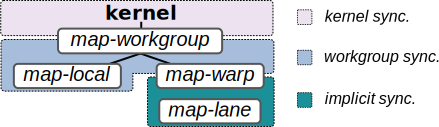
\includegraphics[width=0.8\linewidth]{PACT2014/map}
% \caption{Map hierarchy corresponding to the OpenCL hierarchy. Also shown is the type of synchronization available for each stage.}
% \label{fig:map}
% \end{figure}
% \from{PACT end}
% 
% \from{PPoPP begin}
% \paragraph{Patterns Design and Implementation (PPoPP)}
% \captionsetup[table]{margin=1.75em}
% \begin{table*}[t]
% \centering
% \rowcolors{2}{oddcolor}{evencolor}
% \begin{tabular}{lll}
% \toprule
% \tabhead{Pattern} & \tabhead{Type} & \tabhead{Description}\\
% \midrule
%  %\pat{id}             & $T[n] \rightarrow T[n]$                                & Identity function.\\
%  \pat{map(f)}         & $T[n] \rightarrow U[n], f: T \rightarrow U$            & Apply function $f$ to every element of the input array.\\
%  \pat{reduce(f, z)}   & $T[\ ] \rightarrow T[1], f: (T,T) \rightarrow T, z : T$& Apply the reduction function $f$ with initial value z to the input array.\\
%  %\pat{transpose}      & $T[m][n] \rightarrow T[n][m]$                          & Transpose the 2D input array.\\ 
%  \pat{zip(a,b)}       & $a:T[n], b:U[n] \rightarrow \langle T,U \rangle [n]$   & Zip two arrays into an array of pairs.\\
%  \pat{split}$^n$      & $T[m][\ ]^* \rightarrow T[m/n][n][\ ]^*$               & Splits the outer most dimension of an array in chunks of size n.\\
%  \pat{join}           & $T[m][n][\ ]^* \rightarrow T[m*n][\ ]^*$               & Joins the two outer most dimensions of an array.\\
%  \pat{iterate$^n$(f)} & $T[\ ] \rightarrow T[\ ], f: T[\ ] \rightarrow T[\ ]$  & Iterate the function $f$ over the input $n$ times.\\
%  \pat{reorder}        & $T[n] \rightarrow T[n]$                                & Reorder the element of the input array.\\
% \bottomrule
% \end{tabular}
% \caption{High-level algorithmic patterns used by the programmer. $T \rightarrow U$ means the function input type is $T$ and output type $U$. We write $T[n]$ for an array of type $T$ with size $n$ and $[\ ]^*$ denotes an arbitrary number of dimensions in an array.\vspace{-1em}}
% \label{tab:hlskel}
% \end{table*}
% %
% \begin{table*}[t]
% \centering
% \rowcolors{2}{oddcolor}{evencolor}
% \setlength{\tabcolsep}{2pt}
% \begin{tabular}{lll}
% \toprule
% \tabhead{Pattern} & \tabhead{Type} & \tabhead{Description}\\
% \midrule
%  %\pat{id-primitive}     & $T \rightarrow T$ ($T$ is primitive type)    & Identity function.\\
%  \pat{map-workgroup(f)}    & identical to \pat{map(f)}                     & Each \textbf{workgroup} applies function $f$ on a different element of the input array.\\
%  \pat{map-local(f)}        & identical to \pat{map(f)}                     & Each \textbf{local thread} applies function $f$ on a different element of the input array.\\
%  \pat{map-global(f)}        & identical to \pat{map(f)}                     & Each \textbf{global thread} applies function $f$ on a different element of the input array.\\
%  %\pat{map-warp(f)}         & identical to \pat{map(f)}                     & Each \textbf{warp} applies function $f$ on a different element of the input array.\\
%  %\pat{map-lane(f)}         & identical to \pat{map(f)}                     & Each \textbf{lane thread} applies function $f$ on a different element of the input array.\\
%  \pat{map-seq(f)}          & identical to \pat{map(f)}                     & Apply function $f$ to every element of the input array \textbf{sequentially}.\\
%  \pat{reduce-seq(f,z)}     & identical to \pat{reduce(f,z)}                & Apply reduction function $f$ with initial value z to the input \textbf{sequentially}.\\  
%  \pat{reorder-stride}$^s$  & identical to \pat{reorder}                    & Access input array with a stride $s$ to maintain \textbf{memory coalescing}.\\
%  %\pat{gather(idx, f)} & $T[n] \rightarrow T[n], f: T[n] \rightarrow T[n]$      & The memory index for reading in function $f$ is modified by function $idx$.\\
%  %\pat{scatter(idx, f)}& $T[n] \rightarrow T[n], idx: \code{int} \rightarrow \code{int}$ & The memory index for writing in function $f$ is modified by function $idx$.\\
%  \pat{toLocal(f)}          & $T[\ ] \rightarrow U[\ ], f: T[\ ] \rightarrow U[\ ]$  & Change the storage location for the results of function $f$ to \textbf{local memory}.\\
%  \pat{toGlobal(f)}         & $T[\ ] \rightarrow U[\ ], f: T[\ ] \rightarrow U[\ ]$  & Change the storage location for the results of function $f$ to \textbf{global memory}.\\
%  \pat{asVector}$^n$        & $T[\ ]^*[m] \rightarrow Tn[\ ]^*[m/n]$        & Turns the elements of an array into \textbf{vector type}.\\
%  \pat{asScalar}            & $Tn[\ ]^*[m] \rightarrow T[\ ]^*[m*n]$        & Turns the elements of an array into \textbf{scalar type}.\\
%  \pat{vect}$^n$\pat{(f)}   & $T[n] \rightarrow U[n], f: T \rightarrow U$   & \textbf{Vectorize} the function $f$ by a factor $n$.\\
% \bottomrule
% \end{tabular}
% \caption{Low-level OpenCL patterns used for code generation. The hardware paradigm used is highlighted in bold in the description.}
% \label{tab:llskel}
% \end{table*}
% 
% One of the key ideas of this paper is to expose algorithmic choices and hardware-specific program optimizations as patterns that can be systematically derived using a rule rewriting system (discussed later in in Section~\ref{rules}).
% The high-level algorithmic patterns are designed to be used by the programmer directly.
% The low-level hardware patterns represent hardware specific concepts expressed by a low-level programming model such as OpenCL, the target chosen for this paper.
% Following the same approach, a different set of low-level hardware patterns could be designed to target other low-level programming models such as Pthreads or MPI.
% 
% This section discusses the design of our patterns and how we generate OpenCL code for them.
% We define our patterns as functions which are implicitly applied to exactly one input array and produces one output array.
% To simplify our implementation we decided to encode all types as arrays with primitives represented with arrays of length 1.
% The only exceptions are the user-provided functions such as the \code{mul3} function in Figure~\ref{fig:codeex:map} that operates on a primitive type.
% 
% \subsection{Algorithmic Patterns}
% 
% Table~\ref{tab:hlskel} presents our high-level algorithmic patterns.
% These patterns are not tied to any specific hardware feature and are used to define the program at the algorithmic level by the programmer.
% 
% % \paragraph{Id}
% % The \pat{id} pattern represents the identity function.
% 
% \paragraph{Map}
% The \pat{map} pattern is well known in functional programming and applies a given function $f$ to all elements of its input array.
% 
% \paragraph{Reduce}
% The \pat{reduce} pattern (a.k.a. fold or accumulate) uses a given binary function $f$ to combine all elements of the input array.
% We require the function $f$ to be associative and commutative which allows for an efficient parallel implementation.
% 
% \paragraph{Zip and Split/Join}
% These patterns transform the shape of the data and we store this information, \ie number of dimensions and size of each dimension, in the type system.
% % As a result our code generator does not emit any code for these patterns.
% % The \pat{transpose} pattern simply transposes a 2D array while 
% The \pat{zip} pattern fuses two arrays into an array of pairs.
% The \pat{split} pattern, which is most often combined with a \pat{join}, partitions an array into chunks of specific size resulting in an extra dimension.
% The corresponding \pat{join} pattern does the opposite; it reassembles arrays of arrays by merging dimensions.
% These two patterns used together are similar to the split-join concept from data flow languages such as StreamIt~\cite{thies02streamit}.
%  
% \paragraph{Iterate}
% The \pat{iterate} pattern corresponds to the mathematical definition of iteratively applying a function.
% It is defined as: {$f^0 = id$} and {$f^{n+1} = f^n \circ f$}.
% In terms of implementation, our code generator emits a for-loop to perform the iteration, and two pointers for input and output.
% After each iteration, we swap the pointers, so that the output of the last iteration becomes the input for the next one.
% % We automatically allocated and calculate memory requirements based on the information from the input and output type.
% 
% 
% \paragraph{Reorder}
% 
% The \pat{reorder} pattern is used to specify that the ordering of the elements of an array does not matter.
% This allows our system to reorder arbitrarily the elements of an array and might enable optimizations, as we will see later.
% 
% % The \pat{reorder} pattern allows our system to reorder arbitrarily the elements of an array.
% % In effect, this function can be used to specify that the ordering of the elements of an array does not matter in a given algorithm.
% % No code is generated for this pattern since it is always lowered into low-level hardware patterns according to our rewrite rules.
% 
% 
% \subsection{OpenCL-specific Patterns}
% 
% It is well known, that programming parallel hardware such as manycore CPUs and GPUs is quite complex.
% In order to achieve the highest performance, programmers often use a set of rules of thumb to drive the optimization of their application for the specific devices.
% In fact each hardware vendor provides optimization guides~\cite{nvidia11guide,amd12guide} that extensively cover hardware particularities and how to optimize code for them.
% 
% In this paper we focus on the OpenCL programming model, which is a popular low-level programming model used to program manycore CPUs and GPUs.
% Programming these devices consists of writing a compute \emph{kernel} in OpenCL C that executes on the device and writing the host code that orchestrates data movement, allocates memory and manages the execution on the device.
% 
% We encode the OpenCL programming model by formalizing hardware paradigms expressed as patterns.
% Table~\ref{tab:llskel} gives an overview of the OpenCL-specific patterns we have identified.
% 
% \paragraph{Parallel Maps}
% 
% The different \pat{map} patterns represent possible ways of mapping computations to the hardware and exploit parallelism in OpenCL.
% %For instance, t
% The \pat{map-workgroup(f)} pattern assigns work to a group of threads, called \emph{workgroup} in OpenCL, by letting every workgroup apply the function $f$ on a different element of the input array.
% %Similarly, the other map patterns assign work to local threads inside a workgroup, warps (a bunch of threads being executed simultaneously), or threads inside a warp (lane threads).
% Similarly, the \pat{map-local(f)} pattern assigns work to a local thread inside a workgroup.
% As workgroups are optional in OpenCL the \pat{map-global(f)} pattern assigns work to a global thread, \ie a thread not organized in a workgroup.
% This allows us to map computations in different ways to the thread hierarchy of OpenCL.% as shown in Figure~\ref{fig:map}.
% % One key finding of our paper is that these map patterns are in effect all we need to express parallelism.
% 
% The code generation for all these map patterns is similar, we describe it using \pat{map-workgroup(f)} as an example.
% A loop is generated, where the iteration variable is determined by the \emph{workgroup-id}, which is provided by OpenCL.
% Inside of the loop, a pointer is generated to partition the input array, so that every workgroup processes a different chunk of data.
% We use this pointer as the input for the function $f$ being bound to the map.
% Similarly, we generate and use a pointer for the output.
% After emitting the code for the loop, we continue with the body of the loop by generating the code for the function $f$.
% When the generation of the body is finished, an appropriate synchronization mechanism for the given map pattern is added.
% For instance after a \pat{map-local} we add a barrier synchronization to synchronize the threads inside of the workgroup.
% 
% % An interesting aspect of this approach is that we can automatically optimize away some of the synchronization barriers.
% % On most GPUs, it is possible to avoid synchronization when dealing with threads within the same warp since they are executed in an lock-step synchronized manner (Figure~\ref{fig:map}).
% % As a result the implementation of \pat{map-lane} does not emit any synchronization.
% 
% 
% 
% \paragraph{Sequential Map and Reduce}
% The \pat{map-seq(f)} and \pat{reduce-seq(f,~z)} patterns perform a sequential map and reduction, respectively, within a single thread.
% In both cases the generated code consists of a simple for loop iterating over the array and calling the function $f$.
% In case of the reduction an accumulation variable is initialized with $z$.
% The variable is then passed to the function $f$ in each iteration and the computed result is stored in the accumulation variable and finally written to the output of the reduction.
% 
% \paragraph{Reorder-stride}
% Using this pattern the elements of an array are reordered with a stride $s$.
% In effect, this generates an access to an array such that $out[i] = in[i / n + s \cdot (i \bmod{n})]$, where $n\cdot s$ is the size of the array.
% This hardware pattern ensures that after splitting the workload, consecutive threads access consecutive memory elements (known as a \emph{coalesce memory access}) which is beneficial on modern GPUs as it maximizes the memory bandwidth.
% 
% Our implementation of this pattern does not produce code directly, but generates instead an index function, which is used when accessing the array the next time.
% % Therefore, any following read implicitly reorders the array.
% While not discussed here, our design allows us to support user-defined index functions as well.
% 
% \paragraph{Local/Global}
% The \pat{toLocal(f)} and \pat{toGlobal(f)} patterns are used to determine where the result of function $f$ should be stored.
% OpenCL defines two distinct address spaces: global and local.
% Global memory is the commonly used large but slow memory.
% On GPUs, the small local memory has a high bandwidth with low latency and is used to store frequently accessed data.
% With these two patterns, we can in effect exploit the memory hierarchy defined in OpenCL.
% These patterns act similarly to a typecast and are in fact implemented as such so that no code is emitted directly.
% 
% In our design, every function reads its input and writes its output using pointers provided by the callee function.
% As a result, we can simply force a store to local memory by wrapping any function with our \pat{toLocal} pattern.
% In the code generator, this will simply change the output pointer of function $f$ to an area in local memory.
% 
% \paragraph{Vectorize and asVector/asScalar}
% The OpenCL programming model supports vectorization with special data types such as \code{int4} where any operations on this type will be executed in the hardware vector units.
% In the absence of vector units in the hardware, the OpenCL compiler scalarizes the code automatically.
% 
% The \pat{asVector} and \pat{asScalar} patterns change the data type into vector elements and scalar elements respectively.
% For instance, in OpenCL an array of \code{int} is transformed into an array of \code{int4} as seen in the motivation example (Figure~\ref{fig:codeex}).
% The \pat{vect$^n$(f)} pattern vectorizes a function by simply converting all the operations in $f$ that apply to vector types into vectorized operations. 
% Our current implementation can only vectorize functions containing simple arithmetic operations such as $+$ or $-$.
% In case of more complex functions, we rely on external tools~\cite{garrenberg11vect} for vectorizing the operations. % without performing further analysis.
% \from{PPoPP end}
% 
% \from{PLDI begin}
% \paragraph{Patterns Design and Implementation (PLDI)}
% \captionsetup[table]{margin=1.75em}
% \begin{table*}[t]
% \centering
% \rowcolors{2}{oddcolor}{evencolor}
% \begin{tabular}{ll}
% \toprule
% \tabhead{Pattern} & \tabhead{Description}\\
% \midrule
%  \pat{map(f: $T \rightarrow U$, xs: $T[n]$) $\longrightarrow U[n]$}
%      & Apply function $f$ to every element of the input array $xs$.\\
%  \pat{reduce(f: $(T, T) \rightarrow T$, z: $T$, xs: $T[n]$)} $\longrightarrow T[1]$
%      & Perform a reduction on $xs$ using function $f$ and initial value $z$.\\
%  \pat{zip(xs: $T[n]$, ys: $U[n]$) $\longrightarrow \langle T,U \rangle [n]$}
%      & Zip two arrays into an array of pairs.\\
%  \pat{split}$^n$\pat{(xs: $T[m]$) $\longrightarrow T[n][m/n]$}
%      & Splits the outer most dimension of an array in chunks of size n.\\
%  \pat{join(xs: $T[m][n]$) $\longrightarrow T[m*n]$}
%      & Joins the two outer most dimensions of an array.\\
%  \pat{iterate$^n$(f: $T \rightarrow T$, x: $T$) $\longrightarrow T$}
%      & Iterate the function $f$ over the input $n$ times.\\
%  \pat{reorder(xs: $T[n]$) $\longrightarrow T[n]$}
%      & Reorder the element of the input array $xs$.\\
% \bottomrule
% \end{tabular}
% \caption{High-level algorithmic patterns used by the programmer.
%   $T\rightarrow U$ indicates that the function input type is $T$ and the output type is $U$.
%   We write $T[n]$ for an array of type $T$ with size $n$.\vspace{-1em}}
% \label{tab:hlskel}
% \end{table*}
% %
% \begin{table*}[t]
% \centering
% \rowcolors{2}{oddcolor}{evencolor}
% \setlength{\tabcolsep}{2pt}
% \begin{tabular}{ll}
% \toprule
% \tabhead{Pattern} & \tabhead{Description}\\
% \midrule
%  %\pat{map-\{workgroup | local | global\}(f, xs)}
%  %     & Map $f$ to a \textbf{workgroup}, \textbf{local thread} or \textbf{global thread} respectively.\\
%  \pat{map-workgroup} | \pat{map-local} | \pat{map-global\ (f, xs)}
%       & Map $f$ to a \textbf{workgroup}, \textbf{local thread} or \textbf{global thread} respectively.\\
%  %\pat{map-local(f, xs)}
%  %     & Each \textbf{local thread} applies function $f$ on a different element of the input array.\\
%  %\pat{map-global(f, xs)}
%  %     & Each \textbf{global thread} applies function $f$ on a different element of the input array.\\
%  \pat{map-seq(f, xs)}
%       & Apply function $f$ to every element of the input array \textbf{sequentially}.\\
%  \pat{reduce-seq(f, z, xs)}
%       & Apply reduction function $f$ with initial value z to the input \textbf{sequentially}.\\  
%  \pat{reorder-stride}$^s$\pat{(xs)}
%       & Access input array with a stride $s$ to maintain \textbf{memory coalescing}.\\
%  \pat{toLocal | toGlobal(f: $T[n]\hspace{-.2em}\rightarrow\hspace{-.2em}U[n]$, xs: $T[n]$) $\rightarrow U[n]$}
%       & Store the results of $f$ to \textbf{local} or \textbf{global memory} respectively.\\
%  %\pat{toGlobal(f: $T[\ ] \rightarrow U[\ ]$, xs: $T[\ ]$) $\longrightarrow U[\ ]$}
%  %     & Change the storage location for the results of function $f$ to \textbf{global memory}.\\
%  \pat{asVector}$^n$\pat{(xs: $T[m]$) $\longrightarrow T_n[m/n]$}
%       & Turns the elements of an array into \textbf{vector type}.\\
%  \pat{asScalar(xs: $T_n[m]$) $\longrightarrow T[m*n]$}
%       & Turns the elements of an array into \textbf{scalar type}.\\
%  \pat{vect}$^n$\pat{(f: $T \rightarrow U$) $\longrightarrow (T[n] \rightarrow U[n])$}
%       & \textbf{Vectorize} the function $f$ by a factor $n$.\\
% \bottomrule
% \end{tabular}
% \caption{Low-level OpenCL patterns used for code generation.
%   The hardware paradigm used is highlighted in bold in the description.
%   The types for the first six patterns are identical to the corresponding patterns from Table~\ref{tab:hlskel}.
% }
% \label{tab:llskel}
% \end{table*}
% 
% % \captionsetup[table]{margin=1.75em}
% % \begin{table*}[t]
% % \centering
% % \rowcolors{2}{oddcolor}{evencolor}
% % \begin{tabular}{lll}
% % \toprule
% % \tabhead{Pattern} & \tabhead{Type} & \tabhead{Description}\\
% % \midrule
% %  \pat{map(f, xs)}       & $(T \rightarrow U) \rightarrow T[n] \rightarrow U[n]$
% %                         & Apply function $f$ to every element of the input array $xs$.\\
% %  %\pat{map(f)}         & $T[n] \rightarrow U[n], f: T \rightarrow U$            & Apply function $f$ to every element of the input array.\\
% %  \pat{reduce(f, z, xs)} & $((T,T) \rightarrow T) \rightarrow T \rightarrow T[\ ] \rightarrow T[1]$
% %                         & Perform a reduction on $xs$ using function $f$ and initial value $z$.\\
% %  %\pat{reduce(f, z)}   & $T[\ ] \rightarrow T[1], f: (T,T) \rightarrow T, z : T$& Apply the reduction function $f$ with initial value z to the input array.\\
% %  \pat{zip(xs, ys)}      & $T[n] \rightarrow U[n] \rightarrow  \langle T,U \rangle [n]$
% %                         & Zip two arrays into an array of pairs.\\
% %  %\pat{zip(a,b)}       & $a:T[n], b:U[n] \rightarrow \langle T,U \rangle [n]$   & Zip two arrays into an array of pairs.\\
% %  \pat{split}$^n\pat{(xs)}$ & $T[m] \rightarrow T[n][m/n]$
% %                         & Splits the outer most dimension of an array in chunks of size n.\\
% %  %\pat{split}$^n$      & $T[m][\ ]^* \rightarrow T[m/n][n][\ ]^*$               & Splits the outer most dimension of an array in chunks of size n.\\
% %  \pat{join(xs)}         & $T[m][n] \rightarrow T[m*n]$
% %                         & Joins the two outer most dimensions of an array.\\
% %  %\pat{join}           & $T[m][n][\ ]^* \rightarrow T[m*n][\ ]^*$               & Joins the two outer most dimensions of an array.\\
% %  \pat{iterate$^n$(f, xs)} & $(T \rightarrow T) \rightarrow T[\ ] \rightarrow T[\ ]$  & Iterate the function $f$ over the input $n$ times.\\
% %  %\pat{iterate$^n$(f)} & $T[\ ] \rightarrow T[\ ], f: T[\ ] \rightarrow T[\ ]$  & Iterate the function $f$ over the input $n$ times.\\
% %  \pat{reorder(xs)}        & $T[n] \rightarrow T[n]$                                & Reorder the element of the input array $xs$.\\
% % \bottomrule
% % \end{tabular}
% % \caption{High-level algorithmic patterns used by the programmer. We use the type notation of Haskell and write $T[n]$ for an array of type $T$ with size $n$ and $T[\ ]$ for an array of arbitrary size\vspace{-1em}}
% % \label{tab:hlskel}
% % \end{table*}
% % %
% % \begin{table*}[t]
% % \centering
% % \rowcolors{2}{oddcolor}{evencolor}
% % \setlength{\tabcolsep}{2pt}
% % \begin{tabular}{lll}
% % \toprule
% % \tabhead{Pattern} & \tabhead{Type} & \tabhead{Description}\\
% % \midrule
% %  \pat{map-workgroup(f)}    & identical to \pat{map(f)}                     & Each \textbf{workgroup} applies function $f$ on a different element of the input array.\\
% %  \pat{map-local(f)}        & identical to \pat{map(f)}                     & Each \textbf{local thread} applies function $f$ on a different element of the input array.\\
% %  \pat{map-global(f)}        & identical to \pat{map(f)}                     & Each \textbf{global thread} applies function $f$ on a different element of the input array.\\
% %  \pat{map-seq(f)}          & identical to \pat{map(f)}                     & Apply function $f$ to every element of the input array \textbf{sequentially}.\\
% %  \pat{reduce-seq(f,z)}     & identical to \pat{reduce(f,z)}                & Apply reduction function $f$ with initial value z to the input \textbf{sequentially}.\\  
% %  \pat{reorder-stride}$^s$  & identical to \pat{reorder}                    & Access input array with a stride $s$ to maintain \textbf{memory coalescing}.\\
% %  \pat{toLocal(f)}          & $T[\ ] \rightarrow U[\ ], f: T[\ ] \rightarrow U[\ ]$  & Change the storage location for the results of function $f$ to \textbf{local memory}.\\
% %  \pat{toGlobal(f)}         & $T[\ ] \rightarrow U[\ ], f: T[\ ] \rightarrow U[\ ]$  & Change the storage location for the results of function $f$ to \textbf{global memory}.\\
% %  \pat{asVector}$^n$        & $T[\ ]^*[m] \rightarrow Tn[\ ]^*[m/n]$        & Turns the elements of an array into \textbf{vector type}.\\
% %  \pat{asScalar}            & $Tn[\ ]^*[m] \rightarrow T[\ ]^*[m*n]$        & Turns the elements of an array into \textbf{scalar type}.\\
% %  \pat{vect}$^n$\pat{(f)}   & $T[n] \rightarrow U[n], f: T \rightarrow U$   & \textbf{Vectorize} the function $f$ by a factor $n$.\\
% % \bottomrule
% % \end{tabular}
% % \caption{Low-level OpenCL patterns used for code generation. The hardware paradigm used is highlighted in bold in the description.}
% % \label{tab:llskel}
% % \end{table*}
% 
% The key idea of this paper is to expose algorithmic choices and hardware-specific program optimizations as patterns that are systematically derived using a rule rewriting system (discussed later in Section~\ref{rules}).
% The high-level algorithmic patterns represent structured parallelism.
% They can either be used by the programmer directly as a stand-alone language (or embedded DSL) or used as an intermediate representation targeted by another language.
% Once a program is represented with our high-level patterns, we automatically transform the program into low-level patterns.
% The low-level hardware patterns represent hardware specific concepts expressed by a programming model such as OpenCL, the target chosen for this paper.
% Following the same approach, a different set of low-level patterns could be designed to target other low-level programming models such as Pthreads or MPI.
% 
% 
% \subsection{Algorithmic Patterns}
% 
% We define our patterns as functions. % implicitly applied to exactly one input array and producing one output array.
% To simplify our implementation we encode all types as arrays with primitives represented with arrays of length 1.
% The only exceptions are the user-provided functions such as the \code{mul3} function in Figure~\ref{fig:codeex:map} that operates on a primitive type.
% 
% Table~\ref{tab:hlskel} presents our high-level patterns used to define programs at the algorithmic level.
% Most of the patterns are well known in functional programming, like \pat{map} and \pat{reduce}.
% The \pat{zip}, \pat{split} and \pat{join} patterns transform the shape of the data.
% We store this information, \ie number of dimensions and size of each dimension, in the type system.
% The \pat{iterate} pattern iteratively applies a function multiple times, \eg $f^3 = f \circ f \circ f$. % \ie {$f^0 = id$} and {$f^{n+1} = f^n \circ f$}.
% Finally, the \pat{reorder} pattern lets our system know it is safe to
% reorder the elements of an array arbitrarily, which enables optimizations -- as we will see later.
% 
% %% \paragraph{Map}
% %% The \pat{map} pattern is well known in functional programming and applies a given function $f$ to all elements of its input array.
% %% 
% %% \paragraph{Reduce}
% %% The \pat{reduce} pattern (a.k.a. fold or accumulate) uses a given binary function $f$ to combine all elements of the input array.
% %% We require the function $f$ to be associative and commutative which allows for an efficient parallel implementation.
% %% 
% %% \paragraph{Zip and Split/Join}
% %% These patterns transform the shape of the data and we store this information, \ie number of dimensions and size of each dimension, in the type system.
% %% The \pat{zip} pattern fuses two arrays into an array of pairs.
% %% The \pat{split} pattern, which is most often combined with a \pat{join}, partitions an array into chunks of specific size resulting in an extra dimension.
% %% The corresponding \pat{join} pattern does the opposite; it reassembles arrays of arrays by merging dimensions.
% %% These two patterns used together are similar to the split-join concept from data flow languages such as StreamIt~\cite{thies02streamit}.
% %%  
% %% \paragraph{Iterate}
% %% The \pat{iterate} pattern corresponds to the mathematical definition of iteratively applying a function.
% %% It is defined as: {$f^0 = id$} and {$f^{n+1} = f^n \circ f$}.
% %% In terms of implementation, our code generator emits a for-loop to perform the iteration, and two pointers for input and output.
% %% After each iteration, we swap the pointers, so that the output of the last iteration becomes the input for the next one.
% %% % We automatically allocated and calculate memory requirements based on the information from the input and output type.
% %% 
% %% 
% %% \paragraph{Reorder}
% %% 
% %% The \pat{reorder} pattern is used to specify that the ordering of the elements of an array does not matter.
% %% This allows our system to reorder arbitrarily the elements of an array and might enable optimizations, as we will see later.
% 
% 
% \subsection{OpenCL-specific Patterns}
% 
% Programming manycore CPU and GPU devices is difficult due to the need for managing parallelism, the memory hierarchy and other hardware specific features.
% In order to achieve the highest performance, programmers often use a set of rules of thumb to drive the optimization of their application.
% Each hardware vendor provides optimization guides~\cite{nvidia11guide,amd12guide} that extensively cover hardware particularities and optimizations.
% The main idea behind our work is to identify common optimizations patterns and express them with the help of low-level patterns coupled with
% a rewrite-rule system.
% %
% %In this paper we focus on the OpenCL programming model, which is a popular low-level programming model used to program manycore CPUs and GPUs.
% %Programming these devices consists of writing a compute \emph{kernel} in OpenCL C that executes on the device and writing the host code that orchestrates %data movement, allocates memory and manages the execution on the device.
% Table~\ref{tab:llskel} gives an overview of the OpenCL-specific patterns we have identified.
% 
% \paragraph{Parallel Maps}
% 
% The \pat{map} patterns represent possible ways of mapping computations to the hardware and exploit parallelism in OpenCL.
% %For instance, t
% The \pat{map-workgroup(f, xs)} pattern assigns work to a group of threads, called \emph{workgroup} in OpenCL, with every workgroup applying the function $f$ on an element of the input array.
% %Similarly, the other map patterns assign work to local threads inside a workgroup, warps (a bunch of threads being executed simultaneously), or threads inside a warp (lane threads).
% Similarly, the \pat{map-local} pattern assigns work to a local thread inside a workgroup.
% As workgroups are optional in OpenCL the \pat{map-global} pattern assigns work to a thread not organized in a workgroup.
% This allows us to map computations in different ways to the thread hierarchy.% as shown in Figure~\ref{fig:map}.
% % One key finding of our paper is that these map patterns are in effect all we need to express parallelism.
% 
% The code generation for all these map patterns is similar; we describe it using \pat{map-workgroup} as an example.
% A loop is generated, where the iteration variable is determined by the \emph{workgroup-id} function provided by OpenCL.
% Inside of the loop, a pointer is generated to partition the input array, so that every workgroup calls the function $f$ on a different chunk of data.
% An output pointer is generated similarly.
% We continue with the body of the loop by generating the code for the function $f$ recursively.
% Finally, an appropriate synchronization mechanism for the given map pattern is added.
% For instance after a \pat{map-local} we add a barrier synchronization to synchronize the threads inside of the workgroup.
% 
% % An interesting aspect of this approach is that we can automatically optimize away some of the synchronization barriers.
% % On most GPUs, it is possible to avoid synchronization when dealing with threads within the same warp since they are executed in an lock-step synchronized manner (Figure~\ref{fig:map}).
% % As a result the implementation of \pat{map-lane} does not emit any synchronization.
% 
% 
% 
% \paragraph{Sequential Map and Reduce}
% The \pat{map-seq(f, xs)} and \pat{reduce-seq(f, z, xs)} patterns perform a sequential map and reduction, respectively, within a single thread.
% In both cases the generated code consists of a loop iterating over the array and calling $f$.
% For the reduction an accumulation variable is initialized with $z$ and used to accumulate the results produced by the successive calls to $f$.
% 
% \paragraph{Reorder-stride}
% The elements of array $xs$ are reordered with a stride $s$.
% This generates an access to an array such that $out[i] = in[i / n + s \cdot (i \bmod{n})]$, where $n\cdot s$ is the size of the array.
% This pattern ensures that after splitting the workload, consecutive threads access consecutive memory elements (\ie \emph{coalesce memory access}), which is beneficial on modern GPUs as it maximizes the memory bandwidth.
% 
% Our implementation does not produce code directly, but generates instead an index function, which is used when accessing the array the next time.
% % Therefore, any following read implicitly reorders the array.
% While not discussed here, our design supports user-defined index functions as well.
% 
% \paragraph{Local/Global}
% The \pat{toLocal(f, xs)} and \pat{toGlobal(f, xs)} patterns are used to determine where the result of function $f$ should be stored.
% OpenCL defines two distinct address spaces: global and local.
% Global memory is the commonly used large but slow memory.
% On GPUs, the small local memory has a high bandwidth with low latency and is used to store frequently accessed data.
% With these two patterns, we can in effect exploit the memory hierarchy defined in OpenCL.
% These patterns act similarly to a typecast and are in fact implemented as such so that no code is emitted directly.
% 
% In our design, every function reads its input and writes its output using pointers provided by the callee function.
% As a result, we can simply force a store to local memory by wrapping any function with our \pat{toLocal} pattern.
% In the code generator, this will simply change the output pointer of function $f$ to an area in local memory.
% 
% \newlength{\ruleSpace}
% \setlength{\ruleSpace}{-1em}
% \begin{figure}[t]
% \centering
% % \begin{subfigure}[b]{1\linewidth}
% % \begin{mdframed}
% % $$
% % \begin{array}{lllll}
% %   f & \rightarrow & f \circ \pat{id} & | & \pat{id} \circ f\\
% % \end{array}
% % $$
% % \end{mdframed}
% %   \caption{Identity}
% %   \label{fig:algo:identity}
% % \end{subfigure}
% 
% %\vspace{\ruleSpace}
% \begin{subfigure}[b]{1\linewidth}
% \begin{mdframed}
% $$
% \begin{array}{lrl}
%   \pat{\textbf{iterate}}^{m+n}\pat{(f)} & \rightarrow & \pat{\textbf{iterate}}^m\pat{(f)} \circ \pat{\textbf{iterate}}^n\pat{(f)}\\
%   \end{array}
% $$
% \end{mdframed}
%   \caption{Iterate decomposition}
%   \label{fig:algo:iterate}
% \end{subfigure}
% 
% \vspace{\ruleSpace}
% \begin{subfigure}[b]{1\linewidth}
% \begin{mdframed}
% $$
% \begin{array}{lrl}
%   \pat{map(f)} \circ \pat{reorder} & \rightarrow & \pat{reorder} \circ \pat{map(f)}\\
%   \pat{reorder} \circ \pat{map(f)} & \rightarrow & \pat{map(f)} \circ \pat{reorder}\\  
% \end{array}
% $$
% \end{mdframed}
%   \caption{Reorder commutativity}
%   \label{fig:algo:reorder}
% \end{subfigure}
% 
% \vspace{\ruleSpace}
% \begin{subfigure}[b]{1\linewidth}
% \begin{mdframed}
% $$
% \begin{array}{lrl}
%   \pat{map(f)} & \rightarrow & \pat{\textbf{join}} \circ \pat{map(map(f))}\circ \pat{\textbf{split}}^n
% \end{array}
% $$
% \end{mdframed}
%   \caption{Split-join}
%   \label{fig:algo:splitjoin}
% \end{subfigure}
% 
% \vspace{\ruleSpace}
% \begin{subfigure}[b]{1\linewidth}
% \begin{mdframed}
% \vspace{-.5em}
% $$
% \begin{array}{lrl}
% \pat{reduce(f,z)} & \rightarrow & \pat{reduce(f,z)} \circ \pat{part-red(f,z)}\\[.5em]
% \pat{part-red(f,z)} & \rightarrow & \pat{reduce(f,z)}\\                                                      
%   &| & \pat{part-red(f,z)} \circ \pat{reorder}\\    
%   &| & \pat{\textbf{join}} \circ \pat{map(part-red(f,z))} \circ \pat{\textbf{split}}^n\\
%   &| & \pat{\textbf{iterate}}^{n}\pat{(part-red(f,z))}\\
% \end{array}
% %$$
% %$$
% %\begin{array}{lrl}
% %  \pat{reduce(f,z)} & \rightarrow & \pat{reduce(f,z)} \circ \pat{part-red(f,z)}%\\
% %  %& | & \pat{\textbf{iterate}}^{\infty}\pat{(part-red(f,z))}\\
% %
% %\end{array}
% $$
% \end{mdframed}
%   \caption{Reduction}
%   \label{fig:algo:red}
% \end{subfigure}
% 
% 
% \vspace{\ruleSpace}
% \begin{subfigure}[b]{1\linewidth}
% \begin{mdframed}
% \vspace{-.5em}
% $$
% \begin{array}{lr}
% \pat{\textbf{split}}^n \circ \pat{\textbf{join}}^n \hspace{1em} |\hspace{1em} \pat{\textbf{join}}^n \circ \pat{\textbf{split}}^n & \rightarrow \ \pat{id}\\
% \pat{\textbf{asVector}}^n \circ \pat{\textbf{asScalar}}^n \hspace{.5em} |\hspace{.5em} \pat{\textbf{asScalar}}^n \circ \pat{\textbf{asVector}}^n       & \rightarrow \ \pat{id}\\
% \end{array}
% $$
% \end{mdframed}
%   \caption{Simplification rules}
%    \label{fig:algo:simpl}
% \end{subfigure}
% 
% \vspace{\ruleSpace}
% \begin{subfigure}[b]{1\linewidth}
% \begin{mdframed}
% \vspace{-.5em}
% $$
% \begin{array}{ll}
% \pat{map(f)} \circ \pat{map(g)}                                & \rightarrow \ \ map(f \circ g)\\
% \pat{\textbf{reduce-seq}(f,z)} \circ \pat{\textbf{map-seq}(g)} & \rightarrow \\
% {\hspace{3em}} \pat{\textbf{reduce-seq}}(\lambda\ acc,x:& \hspace{-.75em}f(acc, g(x)), z)\\  % only reduce sequential is valid because non-associativity!!!
% \end{array}
% $$
% \end{mdframed}
%   \caption{Fusion rules}
%    \label{fig:algo:fusion}
% \end{subfigure}
% 
% \vspace{-2em}
% \caption{Algorithmic rules. Bold patterns are known to the code generator.}
% \label{fig:algo}
% \end{figure}
% 
% 
% \paragraph{Vectorize and asVector/asScalar}
% The OpenCL programming model supports vector data types such as \code{int4} where any operations on this type will be executed in the hardware vector units.
% In the absence of vector units in the hardware, the OpenCL compiler scalarizes the code automatically.
% 
% The \pat{asVector} and \pat{asScalar} patterns change the data type into vector elements and scalar elements respectively.
% For instance, an array of \code{int} is transformed into an array of \code{int4} as seen in the motivation example (Figure~\ref{fig:codeex}).
% The \pat{vect$^n$(f)} pattern vectorizes a function by simply converting all the operations in $f$ that apply to vector types into vectorized operations. 
% Our current implementation can only vectorize functions containing simple arithmetic operations. % such as $+$ or $-$.
% In case of more complex functions, we rely on external tools~\cite{garrenberg11vect} for vectorizing the operations. % without performing further analysis.
% \from{PLDI end}

